\documentclass[a4paper, 12pt]{article}

\usepackage[T1]{fontenc}
\usepackage[utf8]{inputenc}
\usepackage[english]{babel}  % ngerman for German
\usepackage{lmodern}  % nicer font
\usepackage{geometry}
\geometry{%
	left   = 2.5cm,
	right  = 2.5cm,
	top    = 3cm,
	bottom = 3cm
}

\usepackage{textcomp}
\usepackage{gensymb}
\usepackage{amsmath,amssymb,amsfonts}
\usepackage{nicefrac}  % nicer inline fractions
\usepackage{tensor}  % allows fancy indices
\usepackage{siunitx}  % easy handling of value + unit (e.g. \SI{10}{\pF})
% \sisetup{}  % configure siunitx (e.g. locale = DE)
\sisetup{output-complex-root=\ensuremath{\mathrm{j}}, complex-root-position = before-number} % configures SI format 10 + j5 for complex numbers (instead of 10 + 5i)

\usepackage{listings}  % code listings
\usepackage{enumerate}
\usepackage{booktabs}  % nicer tables (e.g. \toprule)
\usepackage{verbatim}  % inline code (\verb||)
\usepackage{subcaption}  % captions for subplots
\usepackage[european, siunitx, RPvoltages]{circuitikz}  % draw circuit diagrams
\usepackage{enumitem}
\setlist[itemize]{label=\rule[0.5ex]{0.6ex}{0.6ex}} % black squares for itemize

\usepackage{pstool}  %% Tex fonts in EPS files
\usepackage{graphicx}
\graphicspath{{./figures/}}

\usepackage{etoolbox} % Needed for AtBeginEnvironment command (appendix handling)
\usepackage{appendix} % Appendices environment

\usepackage{csquotes} % removes biber warning
\usepackage[  % ieee style citations (e.g. [1])
	backend     = biber,
	maxbibnames = 99,
	autocite    = footnote,
	style	    = ieee,
	citestyle   = numeric-comp,
	doi=false, isbn=false
]{biblatex}
\addbibresource{bibliography/bibliography.bib}

\usepackage[nobiblatex]{xurl}  % line breaks in URLs
% last imports
\usepackage[bookmarksopen,colorlinks,citecolor=black,linkcolor=black, urlcolor = black]{hyperref}

% after hyperref! 
\usepackage[noabbrev, nameinlink]{cleveref} 
% e.g. \cref{label} or \Cref(label) for capital letter
% configure cleveref not to use brackets around equation references
\creflabelformat{equation}{#2\textup{#1}#3} % Equation references without parentheses
\AtBeginEnvironment{appendices}{\crefalias{section}{appendix}} % Appendix referencing (for cref "Appendix A" instead of "Section A")


% add missing hyphenations
\hyphenation{im-ple-men-ta-tions}

\title{ECS7012P - Music and Audio Programming\\
	   Assignment 1: Synth Filter}
\author{
  Max Tamussino, 200579179
}
\date{\today}


\begin{document}

\maketitle
\tableofcontents
\pagebreak

\section{Introduction} \label{sec:intro}
This report discusses the implementation of a digital emulation of a Moog voltage-controlled filter. The overall structure of this filter is depicted in \Cref{fig:overall-structure}.

\begin{figure}
	\centering
	\includegraphics[width=\textwidth]{overall-structure.jpg}
	\caption{Overall structure of the Moog voltage-controlled filter \cite{Stilson1996}}
	\label{fig:overall-structure}
\end{figure}

\section{First-order filter section} \label{sec:fofs}
As proposed in \cite{Vaelimaeki2006}, one of the four first-order sections of the filter is implemented as depicted in \Cref{fig:first-order-section}. The equations for the individual nodes annotated are given in \Cref{eq:nodes1,eq:nodes2,eq:nodes3,eq:nodes4}. The filter equation was derived from these equations to be \Cref{eq:filter}. By comparing the filter equation the standard form of a first-order IIR filter, which is given in \Cref{eq:first-order-iir}, the filter coefficients $b_0$, $b_1$ and $a_1$ were calculated. The results are given in \Cref{eq:coefficients}.

\begin{figure}
	\centering
	\includegraphics[width=\textwidth]{first-order-section.jpg}
	\caption{First-order section of the filter depicted in \Cref{fig:overall-structure} \cite{Vaelimaeki2006}}
	\label{fig:first-order-section}
\end{figure}

\begin{align}
	\label{eq:nodes1}
	A &= \frac{1}{1.3} \cdot x[n] & B &= x[n-1] \\
	\label{eq:nodes2}
	C &= \frac{0.3}{1.3} \cdot B & D &= A + C \\
	\label{eq:nodes3}
	E &= y[n-1] & F &= D - E \\
	\label{eq:nodes4}
	G &= g \cdot F & y[n] &= E + G
\end{align}

\begin{equation}
	\label{eq:filter}
	y[n] = g \frac{1}{1.3} \cdot x[n] +
	g \frac{0.3}{1.3} \cdot x[n-1] +
	(1-g) \cdot y[n-1]
\end{equation}

\begin{equation}
	\label{eq:first-order-iir}
	y[n] = b_0 \cdot x[n] + 
	b_1 \cdot x[n-1] - 
	a_1 \cdot y[n-1]
\end{equation}

\begin{align}
	\label{eq:coefficients}
	b_0 &= g \frac{1}{1.3} &
	b_1 &= g \frac{0.3}{1.3} &
	a_1 &= g - 1
\end{align}

\subsection{Performance}

The parameter $g$ of the filter coefficients firstly calculated simply by $g = 2 \pi \cdot f_c / f_s$. The filter frequency response using this formula is given in \Cref{fig:prim-resp} for the two different cutoff frequencies. It is clearly visible that the intended cutoff frequencies were not met. In \Cref{subfig:prim-resp-1000}, for $f_c = \SI{1}{\kilo\hertz}$, the response shows its cutoff at approximately \SI{1.1}{\kilo\hertz}, resulting in an error of \SI{10}{\percent}. For $f_c = \SI{4}{\kilo\hertz}$, \Cref{subfig:prim-resp-4000} even shows its cutoff frequency at approximately \SI{5.57}{\kilo\hertz} - an error of \SI{39.3}{\percent}.

\begin{figure} [!ht]
	\centering
	\begin{subfigure}[b]{0.9\textwidth}
		\centering
		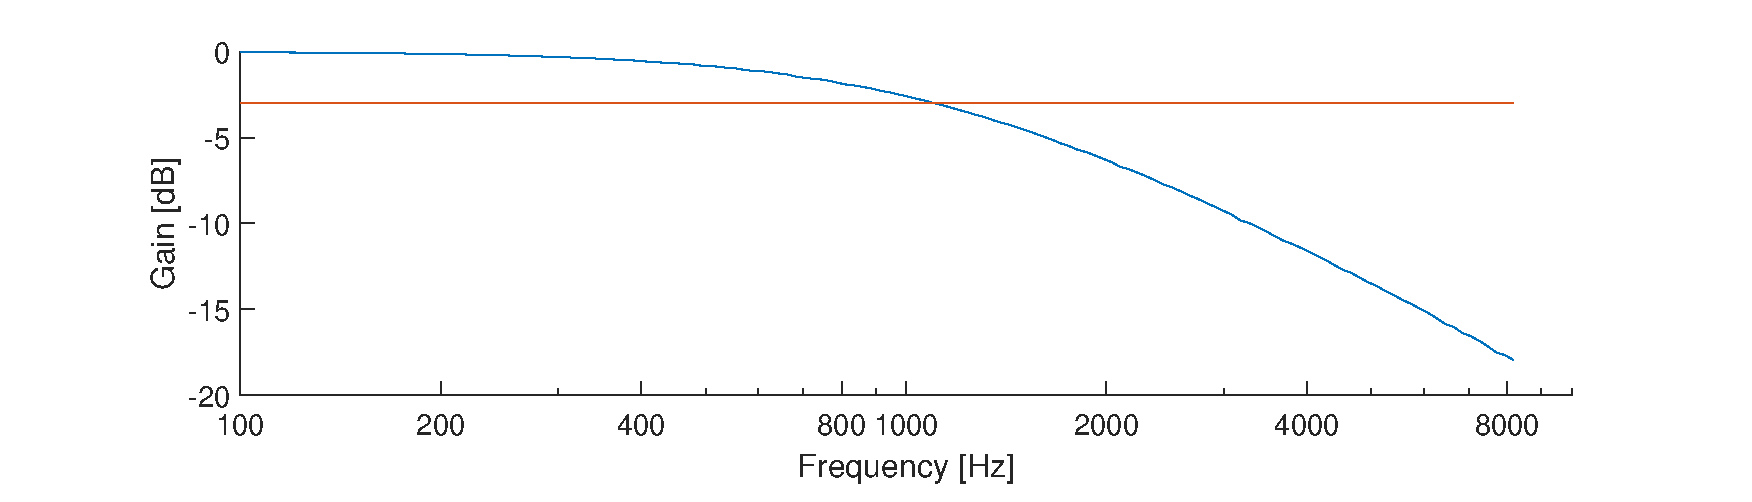
\includegraphics[width=\textwidth]{primitive-response-1000.eps}
		\caption{Response for $f_c = \SI{1}{\kilo\hertz}$}
		\label{subfig:prim-resp-1000}
	\end{subfigure}
	\begin{subfigure}[b]{0.9\textwidth}
		\centering
		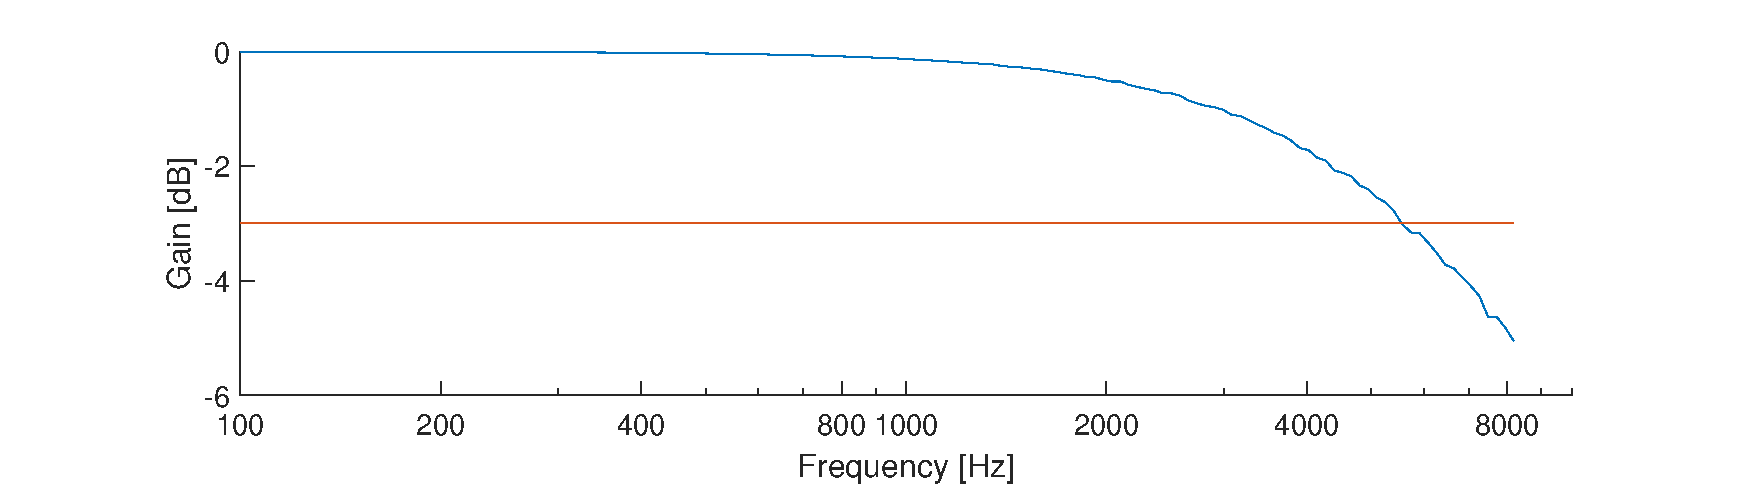
\includegraphics[width=\textwidth]{primitive-response-4000.eps}
		\caption{Response for $f_c = \SI{4}{\kilo\hertz}$}
		\label{subfig:prim-resp-4000}
	\end{subfigure}
	\caption{Filter responses for primitive calculation of parameter $g$}
	\label{fig:prim-resp}
\end{figure}

To mitigate the nonlinear relation of $f_c$ to the actual cutoff frequency, a polynomial model for the parameter $g$ is proposed in \cite{Vaelimaeki2006}. The model is given in \Cref{eq:polynom-fit}, where $\omega_c = 2 \pi \cdot f_c / f_s$. The result for the frequency response of the filter is given in \Cref{fig:ext-resp}. The actual cutoff frequency is around \SI{4.12}{\kilo\hertz}, a significantly improved error of only \SI{3}{\percent}. 

\begin{equation}
	\label{eq:polynom-fit}
	g = 0.9892 \omega_c - 0.4342 \omega_c^2 + 0.1381 \omega_c^3 - 0.0202 \omega_c^4
\end{equation}

\begin{figure}
	\centering
	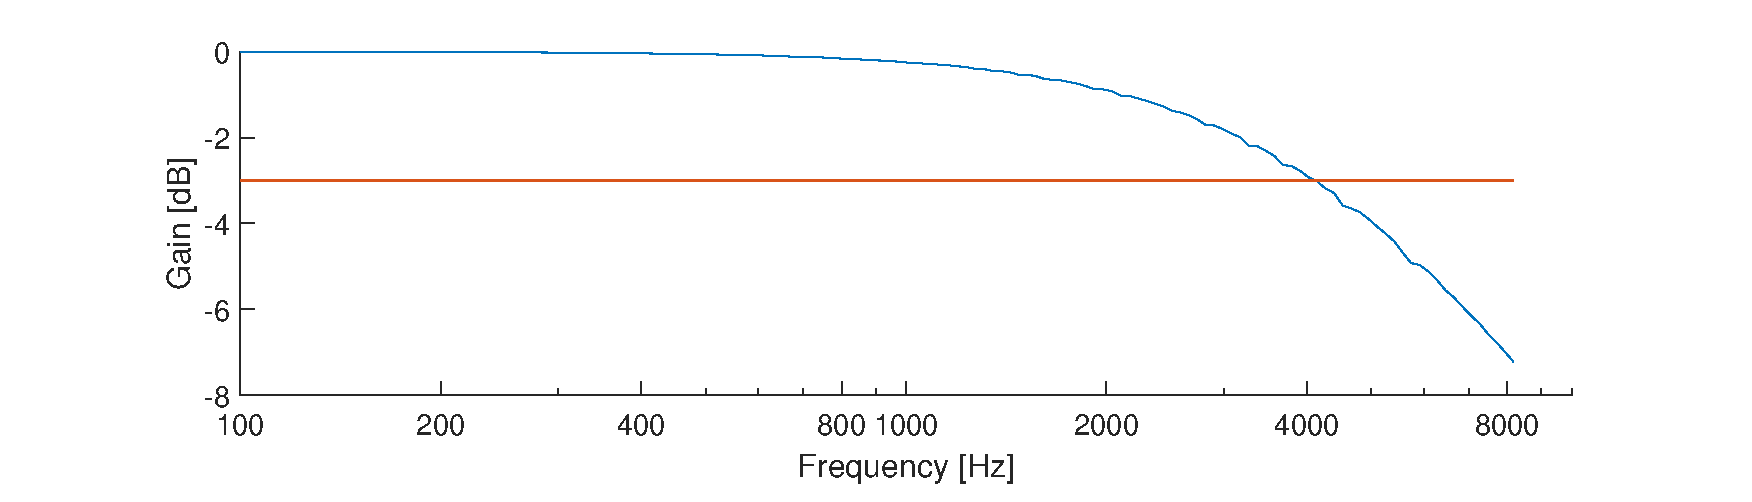
\includegraphics[width=0.9\textwidth]{primitive-response-4000-improved.eps}
	\caption{Filter response for polynomial fit of parameter $g$ (see \Cref{eq:polynom-fit})}
	\label{fig:ext-resp}
\end{figure}

\section{Methods} \label{sec:methods}
\section{Results} \label{sec:results}
\section{Summary and Outlook} \label{sec:summary}

\clearpage
\sloppy
\printbibliography

\end{document}